%%%%%%%%%%%%%%%%%%%%%%%%%%%%%%%%%%%%%%%%%%%%%%%%%%%%%%%%%%%%%%%%%%%%%%
% VM Slides
% February 15, 2016

\documentclass[aspectratio=169]{beamer}
\usepackage{./styles/presentation}

\title{Virtual Memory}
\subtitle{A Project for CS854}

\author[N. Chen, S. Pratt, K. Vaidyanathan]{Nick Chen\\Simon Pratt\\%
Krishna Vaidyanathan}

\date{\today}

\newcommand{\bi}{\begin{itemize}}
\newcommand{\ei}{\end{itemize}}

\newcommand{\bn}{\begin{enumerate}}
\newcommand{\en}{\end{enumerate}}

%%% BEGIN DOCUMENT
\begin{document}

\frame[plain]{\titlepage}

\begin{frame}{Proposal}
  \begin{columns}[T]
    \begin{column}{0.2\textwidth}
    \end{column}
    \begin{column}{0.6\textwidth}
      Our proposal has 3 parts:
      \bn
      \pause
    \item {\color<5>{red} Literature Review}
      \pause
    \item Experimental Design
      \pause
    \item Implementation
      \en
    \end{column}
    \begin{column}{0.2\textwidth}
    \end{column}
  \end{columns}
\end{frame}

\begin{frame}{Proposal: Literature Review}
  \begin{columns}[T]
    \begin{column}{0.4\textwidth}
      We wish to investigate the following operating systems:
      \bn
      \pause
    \item Linux
      \pause
    \item OpenBSD
      \pause
    \item OpenIndiana\\(Previously Solaris)
      \en
    \end{column}
    \begin{column}{0.6\textwidth}
      \pause
    For each OS, we wish to answer the following questions:
    \bi
    \pause
  \item How is physical memory managed?
    \pause
  \item Are there data structures for physical pages, separate from
    the page tables?
    \pause
  \item How are contiguous regions of memory managed?
    \pause
  \item How is memory freed?
    \pause
    \bi
  \item What happens when the kernel runs out of memory?
    \ei
    \pause
  \item Do they do anything special on Non-Uniform Memory Access
    (NUMA) architectures?
    \ei
    \end{column}
  \end{columns}
\end{frame}

\begin{frame}{Proposal}
  \begin{columns}[T]
    \begin{column}{0.2\textwidth}
    \end{column}
    \begin{column}{0.6\textwidth}
      Our proposal has 3 parts:
      \bn
    \item Literature Review
    \item {\color<2>{red} Experimental Design}
    \item Implementation
      \en
    \end{column}
    \begin{column}{0.2\textwidth}
    \end{column}
  \end{columns}
\end{frame}

\begin{frame}{Proposal: Experimental Design}
  \begin{columns}[T]
    \begin{column}{0.2\textwidth}
    \end{column}
    \begin{column}{0.6\textwidth}
      \bi
      \pause
    \item Make a \emph{testable} hypothesis based on lit. review
      \pause
    \item Design \emph{simple} experiments to test this hypothesis
      \ei
    \end{column}
    \begin{column}{0.2\textwidth}
    \end{column}
  \end{columns}
\end{frame}

\begin{frame}{Proposal}
  \begin{columns}[T]
    \begin{column}{0.2\textwidth}
    \end{column}
    \begin{column}{0.6\textwidth}
      Our proposal has 3 parts:
      \bn
    \item Literature Review
    \item Experimental Design
    \item {\color<2>{red} Implementation}
      \en
    \end{column}
    \begin{column}{0.2\textwidth}
    \end{column}
  \end{columns}
\end{frame}

\begin{frame}{Proposal: Implementation}
  \begin{columns}[T]
    \begin{column}{0.2\textwidth}
    \end{column}
    \begin{column}{0.6\textwidth}
      \bi
      \pause
    \item Implement a memory management system for KOS
      \ei
    \end{column}
    \begin{column}{0.2\textwidth}
    \end{column}
  \end{columns}
\end{frame}

\begin{frame}{Progress}
  \begin{columns}[T]
    \begin{column}{0.2\textwidth}
    \end{column}
    \begin{column}{0.6\textwidth}
      We have made some progress:
      \bi
    \item OpenBSD data structures
      \ei
    \end{column}
    \begin{column}{0.2\textwidth}
    \end{column}
  \end{columns}
\end{frame}

\begin{frame}{Progress: OpenBSD}
  \begin{columns}[T]
    \begin{column}{0.4\textwidth}
      \bi
    \item 386BSD\\$\downarrow$\\NetBSD\\$\downarrow$\\OpenBSD
      \pause
    \item VM based on NetBSD
      \pause
      \bi
    \item Rewritten in 1998
      \pause
    \item 270 page PhD dissertation
      \pause
      \ei
      \ei
    \end{column}
    \begin{column}{0.6\textwidth}
      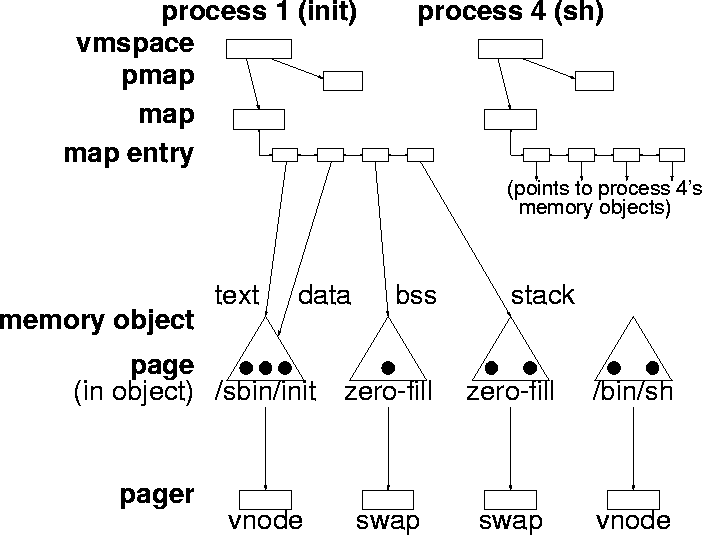
\includegraphics[scale=0.35]{./figures/uvm.png}
    \end{column}
  \end{columns}
\end{frame}

\begin{frame}{Progress: OpenIndiana}
    \begin{enumerate}
        \item Open source fork of OpenSolaris after Oracle take over
        \item Stewarded by the Illumos Foundation
        \item VM uses the ast package by AT\&T, written by Kiem-Phong Vo
        \item Based on paper "Vmalloc: A General and Efficient Memory Allocator"
    \end{enumerate}
\end{frame}

\begin{frame}{Progress: OpenIndiana}
    \begin{enumerate}
        \item Legacy malloc function is old, has shortcomings
        \item malloc not designed for modern environments
        \item Vmalloc a memory allocation library that is flexible and allows a
            wide range of memory operations
            \begin{enumerate}
                \item Regions to organize memory
                \item Obtain memory by application definable disciplines
                \item Customize memory management
            \end{enumerate}
    \end{enumerate}
\end{frame}

\begin{frame}{Summary}
  \begin{columns}[T]
    \begin{column}{0.2\textwidth}
    \end{column}
    \begin{column}{0.6\textwidth}
      \bn
    \item Literature Review
      \bi
    \item Some progress on data structures!
      \ei
    \item Experimental Design
    \item Implementation
      \en
    \end{column}
    \begin{column}{0.2\textwidth}
    \end{column}
  \end{columns}
\end{frame}

\begin{frame}[noframenumbering]{References}
  \small
  \bi
\item UVM dissertation:\\
  \url{http://vorpal.math.drexel.edu/course/opsys2/uvm-project/uvm.pdf}
  \ei
  \bi
  \item Vmalloc: A General and Efficient Memory Allocator:
      \url{http://onlinelibrary.wiley.com/doi/10.1002/\%28SICI\%291097-024X\%28199603\%2926:3\%3C357::AID-SPE15\%3E3.0.CO;2-\%23/abstract}
\ei
\end{frame}

\begin{frame}[noframenumbering]{Attribution}
  \tiny
  \bi
\item OpenBSD data structure diagram from:\\
  \url{http://usenix.org/legacy/publications/library/proceedings/usenix99/full_papers/cranor/cranor_html/index.html}
  \ei
\end{frame}

\begin{frame}[noframenumbering]{License}
  \bi
\item These slides are distributed under the creative commons
  Attribution-ShareAlike 4.0 International (CC BY-SA 4.0).
\item See http://creativecommons.org/licenses/by-sa/4.0/ for details.
  \ei
\end{frame}

\end{document}
